% =====================================================================
%  Designed anisotropy on a manufacturability front:
%  fiber-orientation optimization for elastic stiffness, wave control,
%  and phononic band structure.
%
%  A NEW, self-contained article (separate from dolfinx_wave_control.tex,
%  which is left untouched).  Its thesis --- the fiber-curvature front is
%  the design object, universal across statics / waves / periodic media ---
%  is argued, not surveyed; the bracket, cloak, lens, and metamaterial are
%  evidence for it.
%
%  Elsevier/Springer preprint LOOK: elsarticle.cls / sn-jnl.cls are NOT
%  installed here, so we reproduce the single-column, 11pt, 1.5-spaced
%  preprint layout with base 'article' + setspace + geometry + authblk.
%  Swap in \documentclass{elsarticle} where available.
% =====================================================================
\documentclass[preprint,11pt]{elsarticle}

\usepackage[margin=1in]{geometry}   % override elsarticle's wide preprint margins
\usepackage{setspace}\onehalfspacing
\usepackage{amssymb,amsmath,amsthm}
\usepackage{bm}
\usepackage{booktabs}
\usepackage{algorithm}
\usepackage{algpseudocode}
\usepackage{xcolor}
\usepackage{tikz}
\usepackage{times}
\usetikzlibrary{arrows.meta,positioning,calc}
\tikzset{
  blk/.style={rectangle,rounded corners=2pt,draw=black!65,fill=blue!5,align=center,
              inner sep=4pt,minimum height=8mm,font=\footnotesize,text width=54mm},
  sml/.style={blk,text width=46mm},
  post/.style={blk,fill=green!6},
  ar/.style={-{Latex[length=2mm]},draw=black!70},
  fb/.style={-{Latex[length=2mm]},draw=black!70,dashed},
}
\usepackage[colorlinks=true,allcolors=blue!55!black]{hyperref}

% --- shared result numbers (source of truth, also used by the main paper) ---
\makeatletter
\newcommand{\DefN}[2]{\@ifundefined{\expandafter\@gobble\string#1}{}{}%
  \providecommand#1{}\renewcommand#1{#2}}
\makeatother
\input{results_macros}

% --- light notation ---
\newcommand{\vu}{\mathbf{u}}
\newcommand{\vU}{\mathsf{U}}
\newcommand{\vx}{\mathbf{x}}
\newcommand{\vn}{\mathbf{n}}
\newcommand{\vf}{\mathbf{f}}
\newcommand{\vw}{\mathbf{w}}
\newcommand{\vphi}{\bm{\varphi}}
\newcommand{\veps}{\bm{\varepsilon}}
\newcommand{\vsig}{\bm{\sigma}}
\newcommand{\Tp}{^{\mathsf{T}}}
\newcommand{\Hp}{^{\mathsf{H}}}
\newcommand{\ii}{\mathrm{i}}
\newcommand{\rmd}{\mathrm{d}}
\newcommand{\Df}{\mathbf{D}_f}
\newcommand{\Qf}{\mathbf{Q}_f}
\newcommand{\Tm}{\mathbf{T}}
\newcommand{\Kmat}{\mathbf{K}}
\newcommand{\Mmat}{\mathbf{M}}
\newcommand{\zall}{\zeta_{\mathrm{all}}}
\newcommand{\Real}{\operatorname{Re}}
\newcommand{\Imag}{\operatorname{Im}}

\theoremstyle{plain}\newtheorem{proposition}{Proposition}
\theoremstyle{remark}\newtheorem{remark}{Remark}

\begin{document}
\begin{frontmatter}

\title{Designed anisotropy on a manufacturability front: fiber-orientation optimization
for elastic stiffness, wave control, and phononic band structure}

\author{Joshua R.~Tempelman}
\affiliation{George W.~Woodruff School of Mechanical Engineering, Georgia Institute of Technology, Atlanta GA}

\begin{abstract}
Continuous-fiber composites are among the few directly manufacturable materials whose
anisotropy can be \emph{steered point by point}, making the local fiber orientation a
genuine design field for the material tensor. But a laid tow cannot bend arbitrarily
tightly: automated fiber placement (AFP) imposes a minimum turning radius, so the
fiber-path curvature is bounded. Performance wants sharp steering; manufacturing forbids
it. We show that this single tension organizes fiber-orientation design across
\emph{three} regimes into one object --- a \emph{manufacturability front} of achievable
performance versus allowed tow curvature --- and that the manufacturable design is a
chosen point on that front, never the unconstrained optimum. (i)~\emph{Static stiffness:}
on a fixed topology the optimized fibers reach $\BRANISOPT\%$ of the compliance benefit of
a pointwise-optimal (but unmanufacturable) layup; at the printable end the featured
bracket is $9.4\times$ stiffer than an equal-mass isotropic plate at $0.14\times$ its peak
stress. (ii)~\emph{Wave cloaking}, the sharpest instance: the transformation-elastodynamics
cloak sits at the \emph{singular, unreachable} end of the axis (its material diverges,
Norris) and, imposed on a real fiber, cloaks only $\CLKAN\times$; free optimization
restores the far field $\CLKUNC\times$ but exceeds the print limit; the
curvature-constrained optimum is genuinely printable at $\CLKFEAS\times$. (iii)~\emph{Wave
focusing:} a lens with $\GAINU\times$ focus gain becomes a printable $\GAINC\times$ one.
(iv)~\emph{Periodic media:} fiber orientation on a Bloch cell flattens a chosen band
$\FBFLAT\times$ and opens complete gaps on both sides. The formulation is deliberately
verifiable across all four: a real four-field split of the complex time-harmonic problem,
an automatic discrete adjoint, an \emph{exact isotropy-annihilation identity} the
orientation gradient must satisfy (a built-in correctness certificate) verified to
$\sim\!10^{-6}$, and conforming --- not soft-density --- voids that carry provably zero
interior energy.
\end{abstract}

\begin{keyword}
designed anisotropy \sep fiber-orientation optimization \sep tow-steered composites \sep
manufacturability \sep automated fiber placement \sep elastic wave control \sep
elastic cloaking \sep phononic band gaps \sep adjoint sensitivity
\end{keyword}

\end{frontmatter}

\section{Introduction}
\label{sec:intro}
Tailoring how a solid carries load, propagates waves, or filters vibration is, at
bottom, tailoring its \emph{anisotropy}. The two dominant ways to engineer anisotropy
each pay a manufacturing price. Transformation methods prescribe, exactly, the material
tensor an ideal device would need, but that tensor is usually anisotropic beyond any
ordinary solid and, for elastic waves, is often \emph{singular}: a transformation cloak
requires infinite inertia or an unbounded stiffness ratio at the cloaked
surface~\cite{norris2008,pendry2006}. Metamaterials realize effective anisotropy with
sub-wavelength lattices, inclusions, or local resonators, but the microstructure is
intricate and rarely a solid, load-bearing part.

Continuous-fiber-reinforced polymers occupy a different and underused point. A carbon
tow has a large but \emph{bounded} stiffness contrast (here $E_{f1}/E_{f2}\approx14.6$),
and AFP lets that anisotropy be \emph{oriented locally}, tow by tow, over a solid part.
The orientation field $\theta(\vx)$ is therefore a directly manufacturable design
variable for the material tensor --- what transformation methods ask for, minus the
singularity. The catch is equally physical: a tow has a minimum turning radius $R$, so
the fiber-path curvature obeys $|\zeta|\le\zall=1/R$. \emph{Performance wants sharp
steering; the process forbids it.}

\paragraph{Thesis.} This paper argues that the tension above is not an obstacle to be
tuned away but the \emph{organizing structure} of fiber-orientation design. For a fixed
part it defines a \emph{manufacturability front}: the best achievable performance as a
function of the allowed tow curvature $\zall$, running from gently-steered, easily-printed
designs to a pointwise or transformation ideal that no process reaches. The
manufacturable design is a chosen point on that front. We show the front is the same
object across three physical regimes governed by the \emph{same} rotated fiber tensor
$\Df(\theta)$ --- static stiffness, time-harmonic wave control, and Bloch band structure
--- and that elastic cloaking is its sharpest instance, because there the ideal endpoint
is provably singular and optimization on the front beats the analytical prescription by
roughly five to one.

\paragraph{Contributions.}
\begin{enumerate}\itemsep1pt
\item \textbf{The manufacturability front as a unifying design object}, demonstrated on a
static stiffness/strength bracket, a wave cloak and lens, and a phononic Bloch cell ---
all with one constitutive model, one orientation field, and one curvature constraint
(\S\ref{sec:front},\ref{sec:results}).
\item \textbf{Cloaking as the singular endpoint.} The transformation cloak fails twice for
a real composite: its material is singular, so the fiber curvature diverges and it cannot
be laid; and imposed on a bounded-contrast fiber it cloaks only $\CLKAN\times$. Free
optimization restores the far field $\CLKUNC\times$; the curvature-constrained optimum is
printable at $\CLKFEAS\times$ (\S\ref{sec:cloak}).
\item \textbf{One lever, three physics, one certificate.} A single closed-form
sensitivity, built entirely from $\partial\Df/\partial\theta$, serves the harmonic
adjoint, the compliance adjoint, and the eigenvalue sensitivity; a trigonometric
decomposition of $\Df(\theta)$ yields an \emph{exact isotropy-annihilation identity} the
gradient must satisfy, giving a built-in correctness test (\S\ref{sec:model},\ref{sec:sens}).
\item \textbf{Clean modelling.} A real four-field split of the complex time-harmonic
vector problem, and conforming traction-free voids with provably zero interior energy,
in place of complex arithmetic and soft-density voids (\S\ref{sec:model},\ref{sec:num}).
\end{enumerate}

\paragraph{Relation to prior work.} The manufacturing machinery --- a compactly-supported
radial-basis (CS-RBF) orientation field and a curvature constraint tied to a minimum
turning radius --- is that of Wong, Sanders and Rosen~\cite{wong2025}, whose work designs
\emph{static, maximum-stiffness} parts; we do not claim those ingredients. Elastic
cloaking is well studied: exact transformation theory and its singular material
requirement~\cite{norris2008}; manufacturable \emph{analytical} cloaks for \emph{flexural}
plate waves by affine transformations~\cite{affineCloak}; topology-optimized
\emph{acoustic} cloaks~\cite{toAcoustic}; and single-phase anisotropic elastic
metamaterials by topology optimization~\cite{anisoMeta}. Phononic band gaps are routinely
opened by topology or shape optimization of inclusions. Our contribution is neither the
fiber machinery nor any one device, but the demonstration that \emph{one} manufacturability
front unifies stiffness, wave, and periodic design in a solid steered-fiber medium, with
cloaking as the instance where the ideal is singular and optimization on the front is the
only way to a part one could lay up.

\section{Governing models and the orientation lever}
\label{sec:model}
All three regimes share the plane-stress fiber constitutive law. With the engineering
Voigt strain $\veps(\vu)=[\,\partial_x u_x,\ \partial_y u_y,\ \partial_y u_x+\partial_x
u_y\,]\Tp$, the \emph{rotated} orthotropic stiffness is
\begin{equation}
  \Df(\theta)=\Tm(\theta)\,\Qf\,\Tm(\theta)\Tp,\qquad
  \Tm(\theta)=\begin{bmatrix} c^2 & s^2 & -2sc\\ s^2 & c^2 & 2sc\\
  sc & -sc & c^2-s^2\end{bmatrix},\quad (c,s)=(\cos\theta,\sin\theta),
  \label{eq:Df}
\end{equation}
with $\Qf$ the orthotropic fiber stiffness in material axes (nonzero entries
$Q_{11}=E_{f1}/(1{-}\nu_{12}\nu_{21})$, $Q_{22}=E_{f2}/(1{-}\nu_{12}\nu_{21})$,
$Q_{12}=\nu_{12}Q_{22}$, $Q_{66}=G_{12}$). We use the reference carbon-fiber material
$E_{f1}=131$, $E_{f2}=9$, $G_{12}=5$, $\nu_{12}=0.27$ (contrast $\approx14.6$),
$\rho=1.6$. The scalar signature of the rotated tensor \eqref{eq:Df} is the off-axis
Young's modulus, which it reproduces exactly,
\begin{equation}
  \frac{1}{E_x(\theta)}=\frac{\cos^4\!\theta}{E_{f1}}+\frac{\sin^4\!\theta}{E_{f2}}
  +\Bigl(\frac{1}{G_{12}}-\frac{2\nu_{12}}{E_{f1}}\Bigr)\sin^2\!\theta\cos^2\!\theta ,
  \label{eq:Ex}
\end{equation}
running from $131$ along the fiber to $9$ across (matched to machine precision,
Table~\ref{tab:verify}) --- the anisotropy the optimizer steers. The orientation
$\theta(\vx)$ is the sole design field; the topology is fixed by the device geometry.

\paragraph{Three physics, one tensor.} On a domain $\Omega\subset\mathbb R^2$ we consider:
(i)~time-harmonic in-plane motion $\vu\,e^{-\ii\omega t}$,
\begin{equation}
  -\nabla\!\cdot\!\bigl[(1+\ii\eta)\,\Df(\theta)\veps(\vu)\bigr]
  -\omega^2\rho\,\vu-\ii\,\omega\,c_{\mathrm s}\,\vu=\vf,
  \label{eq:harm}
\end{equation}
with small structural damping $\eta\in[0.02,0.03]$ and an absorbing sponge $c_{\mathrm s}
\ge0$; (ii)~static equilibrium $-\nabla\!\cdot\!(\Df(\theta)\veps(\vu))=\vf$ under a
service load; and (iii)~the clamped generalized eigenproblem $\Kmat(\theta)\vphi=\lambda
\Mmat\vphi$, $\lambda=\omega_n^2$, for natural frequencies. All three carry the design
only through $\Kmat(\theta)=\int_\Omega\veps(\cdot)\Tp\Df(\theta)\veps(\cdot)\,\rmd\vx$.

\paragraph{A trigonometric-polynomial structure.} Expanding \eqref{eq:Df} in $\theta$
gives the exact five-term decomposition
\begin{equation}
  \Df(\theta)=\mathbf C_0+\cos2\theta\,\mathbf C_1+\sin2\theta\,\mathbf C_2
  +\cos4\theta\,\mathbf C_3+\sin4\theta\,\mathbf C_4,
  \label{eq:fourier}
\end{equation}
with the constant $\mathbf C_k$ fixed linear combinations of $Q_{11},Q_{12},Q_{22},
Q_{66}$. Two consequences recur. First, $\partial\Df/\partial\theta=-2\sin2\theta\,\mathbf
C_1+2\cos2\theta\,\mathbf C_2-4\sin4\theta\,\mathbf C_3+4\cos4\theta\,\mathbf C_4$ is
closed form --- no finite differencing of the material tensor. Second, the anisotropy
lives entirely in $\mathbf C_1,\dots,\mathbf C_4$:

\begin{proposition}[Isotropy annihilates the orientation lever]
\label{prop:iso}
If $\Qf$ is isotropic ($Q_{11}=Q_{22}$, $Q_{66}=\tfrac12(Q_{11}-Q_{12})$) then
$\mathbf C_1=\cdots=\mathbf C_4=\mathbf 0$; hence $\Df(\theta)\equiv\mathbf C_0$ and
$\partial\Df/\partial\theta\equiv\mathbf 0$ for every $\theta$.
\end{proposition}
\begin{proof}
The stiffness of an isotropic material is an isotropic tensor, invariant under
$\Tm(\theta)$: $\Tm\Qf\Tm\Tp=\Qf$ for all $\theta$. As \eqref{eq:fourier} holds for all
$\theta$ and $\{1,\cos2\theta,\sin2\theta,\cos4\theta,\sin4\theta\}$ are linearly
independent, matching coefficients forces $\mathbf C_1=\cdots=\mathbf C_4=\mathbf 0$.
\end{proof}

\noindent Because \emph{every} design gradient below is built from
$\partial\Df/\partial\theta$ (\S\ref{sec:sens}), it must vanish identically when the
material is set isotropic --- a one-line exact regression test for any
orientation-sensitivity code, which we use throughout.

\paragraph{Conforming voids.} Wave and structural devices are defined around holes. The
density (SIMP) expedient fills a hole with an ersatz stiffness $E_{\min}$ so the ``void''
still supports a field. We instead mesh every hole \emph{conformingly}: its boundary is a
true traction-free edge and its interior is not part of $\Omega$.

\begin{proposition}[Void energy]
\label{prop:void}
For a hole $V$ with traction-free boundary excluded by conforming meshing, the elastic and
kinetic energy stored in $V$ is exactly zero. If instead $V$ is retained with ersatz
stiffness $E_{\min}$ and mass $\rho_{\min}$, the interior field is generically nonzero and
the spurious energy is $O(E_{\min})$, polluting any objective or gradient integrated over a
region overlapping $V$.
\end{proposition}
\noindent Conforming exclusion makes $V\cap\Omega=\varnothing$, so no degrees of freedom
live in $V$; for soft-void the interior strain energy scales linearly with $E_{\min}$.
A soft-void cloak can thus report cloaking that is partly the ersatz interior cancelling
itself. All results below use conforming voids.

\section{One lever, three physics: sensitivities}
\label{sec:sens}
Discretizing any of the three models gives a linear (or generalized-eigen) problem whose
design dependence is confined to $\Kmat(\theta)$. Each objective's gradient reduces to a
single bilinear form in $\partial\Df/\partial\theta$, so Proposition~\ref{prop:iso}
applies to all three.

\paragraph{Harmonic (cloak, lens).} A lens maximizes the energy in a focal region,
$E=\int_{\Omega_{\rm reg}}|\vu|^2\,\rmd\vx$; a cloak minimizes the far-field mismatch to a void-free
reference, $J=\int_{\Omega_{\rm obs}}|\vu-\vu_{\rm ref}|^2\,\rmd\vx$. Both are quadratic in the
discrete state $\vU$. Adjoin the forward problem $\mathcal A(\theta)\vU-\vf=\mathbf 0$ with
a multiplier $\bm\Lambda$, $\mathcal L=J(\vU)+\bm\Lambda\Tp(\mathcal A\vU-\vf)$; on the
constraint manifold $\mathcal L=J$, and the total derivative separates into implicit and
explicit parts,
\begin{equation}
  \frac{\rmd J}{\rmd\theta_\ell}
  =\underbrace{\Bigl(\tfrac{\partial J}{\partial\vU}+\mathcal A\Tp\bm\Lambda\Bigr)\Tp
  \tfrac{\rmd\vU}{\rmd\theta_\ell}}_{\text{eliminated by the adjoint}}
  +\ \bm\Lambda\Tp\frac{\partial\mathcal A}{\partial\theta_\ell}\vU .
  \label{eq:lagr}
\end{equation}
Choosing $\bm\Lambda$ to annihilate the implicit-state term gives the discrete adjoint
equation $\mathcal A(\theta)\Tp\bm\Lambda=-\partial J/\partial\vU$, after which the design
derivative is the explicit $\theta$-dependence of the residual alone. Writing the
$\theta$-derivative bilinear form $b(\vu,\vw)\equiv\veps(\vu)\Tp(\partial\Df/\partial\theta)
\veps(\vw)$ and using that only stiffness carries $\theta$,
\begin{equation}
  \frac{\rmd J}{\rmd\theta_\ell}=\int_{\Omega_\ell}\Bigl[
  b(\vu_r,\bm\lambda_r)+b(\vu_i,\bm\lambda_i)
  +\eta\bigl(b(\vu_r,\bm\lambda_i)-b(\vu_i,\bm\lambda_r)\bigr)\Bigr]\,\rmd\vx,
  \label{eq:sensharm}
\end{equation}
with $(\vu_r,\vu_i),(\bm\lambda_r,\bm\lambda_i)$ the real/imaginary state and adjoint. The
adjoint is driven by the objective's state-gradient $\partial J/\partial\bar{\vU}$: with the
region Gram matrix $\Mmat_R=\int_{\Omega_R}\mathbf N\Tp\mathbf N$, the focal-energy objective
$E=\vU\Hp\Mmat_{\rm reg}\vU$ that the lens \emph{maximizes} ($J=-E$) has load
$-\Mmat_{\rm reg}\vU$ --- simply the state restricted to the focal region, so the lens is
self-adjoint up to that restriction --- while the cloak mismatch $J=(\vU-\vU_{\rm ref})\Hp
\Mmat_{\rm obs}(\vU-\vU_{\rm ref})$ has load $\Mmat_{\rm obs}(\vU-\vU_{\rm ref})$. The adjoint
solve reuses the transposed forward factorization, so it adds no assembly.

\paragraph{Compliance (stiffness).} Minimizing the service compliance $c=\vf\Tp\vu$ is
self-adjoint, so
\[
  \rmd c/\rmd\theta_\ell=-\int_{\Omega_\ell}\veps(\vu)\Tp(\partial\Df/\partial\theta)
  \veps(\vu)\,\rmd\vx .
\]

\paragraph{Eigenfrequency (dynamics).} For a simple eigenvalue $\lambda_n=\omega_n^2$
with a mass-normalized mode $\vphi_n$ ($\vphi_n\Tp\Mmat\vphi_n=1$), first-order (Rayleigh
-quotient) perturbation gives the design derivative
\begin{equation}
  \frac{\partial\lambda_n}{\partial p}=\vphi_n\Tp\Bigl(\frac{\partial\Kmat}{\partial p}
  -\lambda_n\frac{\partial\Mmat}{\partial p}\Bigr)\vphi_n,
  \qquad p\in\{\theta_\ell,\ z_e\},
  \label{eq:eigsens}
\end{equation}
requiring no eigenvector derivative --- the eigenvector's projection onto its own mode
cannot change the quotient to first order. This is the identical generalized-eigenproblem
sensitivity used throughout the companion study; the two settings here are just
specializations. For an \emph{orientation} variable only the stiffness carries the design
($\partial\Mmat/\partial\theta=0$), so \eqref{eq:eigsens} collapses to the strain-energy
form $\rmd\lambda_n/\rmd\theta_\ell=\int_{\Omega_\ell}\veps(\vphi_n)\Tp(\partial\Df/\partial
\theta)\veps(\vphi_n)\,\rmd\vx$; a \emph{density} variable additionally contributes the mass
term $-\lambda_n(\rho_f-\rho_m)\,\vphi_n\Tp\mathbf m_e\vphi_n$. The reading is clean ---
change in the mode's \emph{strain} energy minus $\lambda_n$ times the change in its
\emph{kinetic} energy --- so a natural frequency rises when a perturbation stiffens the mode
faster than it mass-loads it, and falls otherwise; everything follows from the one eigenpair
already computed. The periodic (Bloch) band-structure sensitivity in \S\ref{sec:meta} is the
same expression with $\vphi_n$ replaced by the reduced Bloch mode $\bm\psi_n=\mathbf T(\mathbf k)
\vphi_n$ and $\Tp\!\to\!{}\Hp$.

\paragraph{Peak stress (strength).} The bracket's strength is governed by a $p$-norm
surrogate of the peak von Mises stress,
\begin{equation}
  \Sigma_p=\Bigl(\sum_e\tfrac{A_e}{\sum_k A_k}\,\tilde\sigma_e^{\,p}\Bigr)^{1/p},\qquad
  \tilde\sigma_e=z_e^{\,q}\sqrt{\bm\sigma_e\Tp\mathbf V\bm\sigma_e},\quad
  \bm\sigma_e=\Df(\theta_e)\,\mathbf B_e\vu_e,
  \label{eq:pnorm}
\end{equation}
with $\mathbf V$ the plane-stress von Mises matrix and $z_e^{\,q}$ ($q=\tfrac12$) a
qp-relaxation that stops void elements carrying spurious stress. Its derivative has an
explicit part (the element stress depends on $\theta$ through $\Df$) and an implicit part
through $\vu$; the latter is a single adjoint solve $\Kmat\bm\mu=\partial\Sigma_p/\partial
\vu$ reusing the static factorization, so $\partial\Sigma_p/\partial\theta_\ell=
\partial\Sigma_p/\partial\theta_\ell|_{\rm expl}-\bm\mu\Tp(\partial\Kmat/\partial\theta_\ell)
\vu$, again a $\partial\Df/\partial\theta$ form. Both stress derivatives pass the
finite-difference check to $\lesssim10^{-7}$.

\medskip
\noindent Each of \eqref{eq:sensharm} and its static/modal counterparts is built
\emph{only} from $\partial\Df/\partial\theta$; setting the material isotropic must return
an identically zero gradient (Proposition~\ref{prop:iso}). We verify the non-trivial
gradients against central finite differences to $\sim\!10^{-6}$ and the isotropy identity
to machine precision (Table~\ref{tab:verify}).

\section{Manufacturability, and the front}
\label{sec:front}
\paragraph{Smooth orientation field.} A raw per-cell orientation is mesh-scale noisy ---
unmanufacturable and, driving a wave field, incoherent. We parametrize $\theta$ by a coarse
grid of support-point angles $\hat\theta=\{\hat\theta_i\}$ at sites $\{\mathbf s_i\}$
(spacing $h_s$), interpolated to the cell centroids $\{\vx_c\}$ by a compactly-supported
Wendland $C^2$ radial basis $\phi(q)=(1-q)^4(4q+1)$ (support $q<1$):
\begin{equation}
  \theta_c=(\mathbf B\hat\theta)_c=\sum_i B_{ci}\hat\theta_i,\qquad
  B_{ci}=\frac{\phi(q_{ci})}{\sum_j\phi(q_{cj})},\qquad
  q_{ci}=\frac{\lVert\vx_c-\mathbf s_i\rVert}{r},
  \label{eq:rbf}
\end{equation}
a row-stochastic map ($\sum_i B_{ci}=1$). By the chain rule the design gradient is a single
transpose apply, $\partial J/\partial\hat\theta=\mathbf B\Tp(\partial J/\partial\theta)$.
The support radius $r$ --- not the mesh $h$ --- sets the finest resolvable fiber curvature,
so the constraint below is mesh-independent, and the design is low-dimensional and smooth
\emph{by construction}. Where the device is mirror-symmetric (the lens about $y=L_y/2$) we
enforce it exactly: a director is symmetric iff $\theta(x,L_y{-}y)=-\theta(x,y)$, so we use a
symmetric support grid and project $\hat\theta\mapsto\tfrac12(\hat\theta-\hat\theta_{\rm
mirror})$ each iteration, removing the spurious asymmetry the triangulation would otherwise
introduce.

\paragraph{Fiber-path curvature.} A printable tow has minimum turning radius $R$. The
relevant quantity is the curvature of the fiber \emph{streamline}: the directional
derivative of $\theta$ along the fiber $\vn=(\cos\theta,\sin\theta)$,
\begin{equation}
  \zeta(\vx)=(\vn\!\cdot\!\nabla)\theta=\cos\theta\,\partial_x\theta+\sin\theta\,
  \partial_y\theta,\qquad |\zeta(\vx)|\le\zall=\tfrac1R .
  \label{eq:curl}
\end{equation}
The spatial gradients come \emph{analytically} from the map \eqref{eq:rbf}: writing
$W_{ci}=\phi(q_{ci})$, $S_c=\sum_j W_{cj}$ and differentiating the kernel \emph{and} its
normalization consistently,
\begin{equation}
  (\mathbf B_x)_{ci}=\frac{\partial_x W_{ci}}{S_c}-B_{ci}\frac{\sum_j\partial_x W_{cj}}{S_c},
  \qquad
  \partial_x W_{ci}=-\frac{20\,q_{ci}(1-q_{ci})^3}{r}\,\frac{x_c-s_{ix}}{\lVert\vx_c-\mathbf
  s_i\rVert},
  \label{eq:rbfderiv}
\end{equation}
and likewise $\mathbf B_y$ (using $\phi'(q)=-20\,q(1-q)^3$), so $\partial_x\theta=\mathbf
B_x\hat\theta$, $\partial_y\theta=\mathbf B_y\hat\theta$, and both $\zeta$ and
$\partial\zeta/\partial\hat\theta$ are exact --- no finite differencing of the curvature.

\paragraph{From orientation to laid tows.} The orientation field is delineated into
finite-pitch \emph{toolpaths} by the wave-projection scheme: from the sign-free
double-angle director $(\cos2\theta,\sin2\theta)$ a seam-free branch of $\theta$ is
recovered by region-growing sign propagation, and a phase field $\psi$ is solved for whose
gradient is unit and orthogonal to the fibers,
\begin{equation}
  \psi=\arg\min_\psi\!\int_\Omega\bigl\lVert\nabla\psi-[-\sin\theta,\ \cos\theta]\Tp
  \bigr\rVert^2\,\rmd\vx ,
  \label{eq:phase}
\end{equation}
matched \emph{directly} (a gradient least-squares, not the normal-equations Poisson form,
which would collapse the pitch). The evenly-spaced level sets of $\psi$ --- the peaks of
$\chi=\tfrac12+\tfrac12\cos(2\pi\psi/d)$ --- are the as-manufactured tows at pitch $d$; they
follow the fiber direction, keep a fixed spacing, and are masked out of every void, so no
tow crosses a hole. The tow figures in \S\ref{sec:results} are these level sets.

\paragraph{The front.} We impose \eqref{eq:curl} with a smooth one-sided penalty
$\Pi=\langle\max(0,\zeta^2-\zall^2)\rangle$ and compose the total gradient by pulling the
objective sensitivity back through the CS-RBF transpose and balancing it against the
curvature penalty,
\begin{equation}
  \mathbf g=\mathbf B\Tp\frac{\partial\mathcal J}{\partial\theta}
  +\mu\,\frac{\lVert\mathbf B\Tp\partial\mathcal J/\partial\theta\rVert}
  {\lVert\partial\Pi/\partial\hat\theta\rVert}\,\frac{\partial\Pi}{\partial\hat\theta},
  \label{eq:gcompose}
\end{equation}
with the penalty pre-scaled to the objective-gradient norm. The weight $\mu$ is adapted
toward the limit --- raised while $\max|\zeta|>\zall$, eased otherwise --- and the best
iterate that is actually feasible ($\max|\zeta|\le\zall$) is retained, so the reported
design is guaranteed printable (Algorithm~\ref{alg:opt}, Figure~\ref{fig:flow}). Sweeping
$\zall$ is an $\varepsilon$-constraint traversal of the performance--curvature Pareto: the
\emph{manufacturability front}, whose far ($\zall\!\to\!\infty$) end is the unconstrained
optimum (or, in the cloak, the singular transformation ideal) and whose near end is the
gently-steered, easily-printed design. The curve --- not any single optimum --- is the
design object.

\paragraph{Optimizer.} Each step, the Method of Moving Asymptotes replaces $\mathcal J$ and
$\Pi$ by convex separable approximations built from moving asymptotes $L_\ell<\hat\theta_\ell
<U_\ell$ that contract or expand by the sign history of $\hat\theta_\ell$, with a per-step
move limit; the box $|\hat\theta_\ell|\le\tfrac\pi2$ reflects the director periodicity. Because
raw wave objectives are $O(10^{-4})$, we feed MMA the scale-invariant log-gradient
$\partial_\theta\ln E$ (lens) or $\partial_\theta\ln J$ (cloak).

\begin{algorithm}[htbp]
\caption{Curvature-constrained fiber-orientation design (best-feasible; cf.\
Figure~\ref{fig:flow})}
\label{alg:opt}
\begin{algorithmic}[1]
\Require mesh with conforming voids, material $\Qf$, objective (harmonic / static / eigen),
  curvature limit $\zall$, support sites $\{\mathbf s_i\}$ and radius $r$
\State build $\mathbf B,\mathbf B_x,\mathbf B_y$ \eqref{eq:rbf}--\eqref{eq:rbfderiv} and the
  symmetry projector $\mathbf S$; \ $\hat\theta\gets\mathbf 0$ \Comment{straight-fiber baseline}
\State (cloak only) solve the void-free reference $\vu_{\rm ref}$ on the same mesh
\For{$\mu\in\{\mu_0,\dots,\mu_{\max}\}$} \Comment{adaptive penalty continuation}
  \For{$t=1,\dots,T$}
    \State $\hat\theta\gets\mathbf S\hat\theta$; \ $\theta\gets\mathbf B\hat\theta$
      \Comment{symmetrize, then interpolate}
    \State assemble $\mathcal A(\theta)$ (real $4$-field \eqref{eq:block}) \emph{or}
      $\Kmat,\Mmat$; factor, and \textbf{solve} the state
    \State evaluate $\mathcal J$; \textbf{adjoint}
      $\mathcal A\Tp\bm\Lambda=-\partial\mathcal J/\partial\vU$ \Comment{reuse factors}
    \State $\partial\mathcal J/\partial\theta\gets$
      \eqref{eq:sensharm}\,/\,\eqref{eq:eigsens}\,/\,\eqref{eq:pnorm}
      \Comment{a $\partial\Df/\partial\theta$ form}
    \State $\zeta\gets\cos\theta\,\mathbf B_x\hat\theta+\sin\theta\,\mathbf B_y\hat\theta$;
      \ $\mathbf g\gets$ \eqref{eq:gcompose}; \
      $\hat\theta\gets\textsc{MMA}(\hat\theta,\mathbf g;\ |\hat\theta|\le\tfrac\pi2)$
  \EndFor
  \State retain the best feasible iterate; \textbf{if} $\max_c|\zeta_c|\le\zall$
    \textbf{break} \Comment{printable}
\EndFor
\State \textbf{delineate toolpaths} \eqref{eq:phase}; \Return best design, fields, and tows
\end{algorithmic}
\end{algorithm}

\begin{figure}[htbp]
\centering
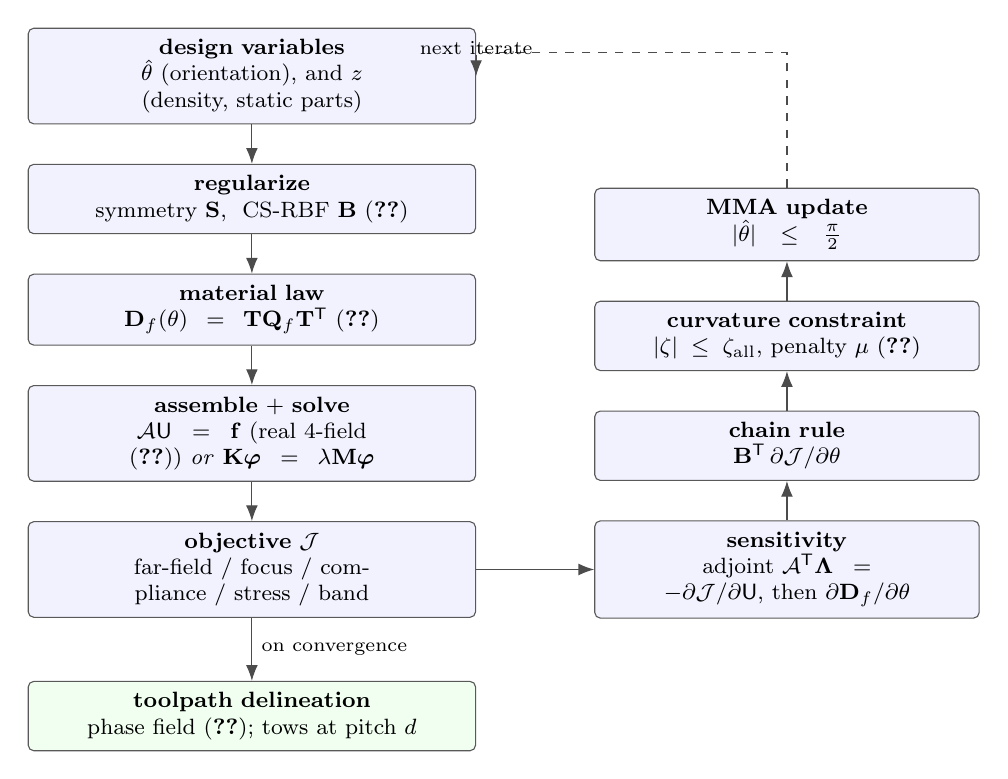
\begin{tikzpicture}[node distance=5mm and 15mm]
\node[blk] (des) {\textbf{design variables}\\ $\hat\theta$ (orientation), and $z$ (density,
  static parts)};
\node[blk,below=of des] (reg) {\textbf{regularize}\\ symmetry $\mathbf S$, \ CS-RBF
  $\mathbf B$ \eqref{eq:rbf}};
\node[blk,below=of reg] (mat) {\textbf{material law}\\
  $\Df(\theta)=\Tm\Qf\Tm\Tp$ \eqref{eq:Df}};
\node[blk,below=of mat] (asm) {\textbf{assemble $+$ solve}\\ $\mathcal A\vU=\vf$ (real
  $4$-field \eqref{eq:block}) \emph{or} $\Kmat\vphi=\lambda\Mmat\vphi$};
\node[blk,below=of asm] (obj) {\textbf{objective $\mathcal J$}\\ far-field / focus /
  compliance / stress / band};
\node[sml,right=of obj] (sens) {\textbf{sensitivity}\\ adjoint
  $\mathcal A\Tp\bm\Lambda=-\partial\mathcal J/\partial\vU$, then $\partial\Df/\partial\theta$};
\node[sml,above=of sens] (chain) {\textbf{chain rule}\\
  $\mathbf B\Tp\,\partial\mathcal J/\partial\theta$};
\node[sml,above=of chain] (con) {\textbf{curvature constraint}\\ $|\zeta|\le\zall$,
  penalty $\mu$ \eqref{eq:gcompose}};
\node[sml,above=of con] (mma) {\textbf{MMA update}\\ $|\hat\theta|\le\tfrac\pi2$};
\node[post,below=8mm of obj] (tp) {\textbf{toolpath delineation}\\ phase field
  \eqref{eq:phase}; tows at pitch $d$};
\draw[ar] (des)--(reg); \draw[ar] (reg)--(mat); \draw[ar] (mat)--(asm); \draw[ar] (asm)--(obj);
\draw[ar] (obj)--(sens); \draw[ar] (sens)--(chain); \draw[ar] (chain)--(con); \draw[ar] (con)--(mma);
\draw[fb] (mma.north) |- ($(des.east)+(0,3mm)$) -- (des.east)
  node[midway,above,font=\scriptsize] {next iterate};
\draw[ar] (obj)--(tp) node[midway,right,font=\scriptsize] {on convergence};
\end{tikzpicture}
\caption{\textbf{Data flow of the design loop.} Left column: design variables descend
through the regularization operators into the material law, the assembled operator, and the
solve. Right column: the gradient ascends through the adjoint (wave, compliance, stress) or
eigenvalue perturbation (modal, band), then the \emph{transpose} of the CS-RBF map and the
curvature constraint, to the MMA update, which returns the next iterate (dashed). Green: the
toolpath delineation that turns the converged orientation field into printable tows.}
\label{fig:flow}
\end{figure}

\section{Numerical formulation and verification}
\label{sec:num}
\paragraph{Real four-field split.} The weak form of \eqref{eq:harm} is complex-symmetric,
$[(1+\ii\eta)\Kmat-\omega^2\Mmat+\ii\omega\mathbf C]\vu=\vf$. Writing the complex operator
as $A+\ii B$ with $A=\Kmat-\omega^2\Mmat$ and $B=\eta\Kmat+\omega\mathbf C$ both real
symmetric, and $\vu=\vu_r+\ii\vu_i$, the equivalent real block system on
$(u_{xr},u_{yr},u_{xi},u_{yi})$ is
\begin{equation}
  \begin{bmatrix} A & -B\\ B & \phantom{-}A\end{bmatrix}
  \begin{bmatrix}\vu_r\\ \vu_i\end{bmatrix}=\begin{bmatrix}\vf_r\\ \vf_i\end{bmatrix},
  \label{eq:block}
\end{equation}
solved by a real \texttt{PETSc} build. Block \eqref{eq:block} is exactly
$[\Real,-\Imag;\Imag,\Real]$ of the complex operator: expanding
$(A+\ii B)(\vu_r+\ii\vu_i)=(A\vu_r-B\vu_i)+\ii(B\vu_r+A\vu_i)\overset{!}{=}\vf_r+\ii\vf_i$
and equating real and imaginary parts separately gives the two coupled real systems, so no
complex arithmetic is needed and the structural damping $\eta\Kmat$ joins the sponge in the
off-diagonal block. The elements are conforming constant-strain triangles; every hole is
meshed as a true boundary (Proposition~\ref{prop:void}) with \texttt{gmsh}, not a soft
inclusion on a structured grid --- staircased boundaries would scatter the wave and corrupt
the gradient.

\paragraph{Truncation, drive, and reference.} A finite plate is made to radiate as if
unbounded by a mass-proportional sponge $c_{\mathrm s}(\vx)$ that ramps quadratically into
a margin of width $m$ on the three non-driven edges,
\begin{equation}
  c_{\mathrm s}(\vx)=c_0\Bigl[\max\Bigl(0,\ \tfrac{x-(L_x-m)}{m},\ \tfrac{m-y}{m},\
  \tfrac{y-(L_y-m)}{m}\Bigr)\Bigr]^2 ,
  \label{eq:sponge}
\end{equation}
driven by an $x$-directed line source $\vf=(A\,e^{-\beta(x-x_0)^2},0)$ near the left edge (a
plane pressure wave). Because $\Mmat$, the sponge $\mathbf C$, and $\vf$ carry no $\theta$,
they drop out of every sensitivity \eqref{eq:sensharm}. The cloak reference $\vu_{\rm ref}$
is the field solved on the \emph{same} mesh with the void filled --- the wave that would
exist with no hole --- so $J$ measures exactly the scattering the void introduces.
Table~\ref{tab:params} lists the constants.

\begin{table}[htbp]
\centering\small
\caption{Model and design parameters (nondimensional units).}
\label{tab:params}
\begin{tabular}{@{}llll@{}}
\toprule
Group & Parameter & Cloak / lens & Bracket\\
\midrule
Material & $E_{f1},E_{f2},G_{12},\nu_{12}$ & \multicolumn{2}{l}{$131,\ 9,\ 5,\ 0.27$
  \quad($\rho=1.6$)}\\
Damping & structural $\eta$ & \multicolumn{2}{l}{$0.02$--$0.03$}\\
Wave & frequency $\omega$; source $(A,\beta,x_0)$ & $50$; $(30,80,0.1)$ & ---\\
Sponge & $(c_0,m)$ & $(80,0.6)$/$(70,0.55)$ & ---\\
Domain & $(L_x,L_y)$ & $(8,5)$ & $(3.5,2.0)$\\
Cloak void & $R_V$, design shell $R_{\rm des}$ & $0.55,\ 1.5$ & ---\\
Orientation & CS-RBF spacing $h_s$, radius $r$ & $(0.33,0.7)$/$(0.28,0.6)$ & $0.045$--$0.06$\\
Curvature & limit $\zall=1/R$ & swept & $9$ (featured)\\
\bottomrule
\end{tabular}
\end{table}

\paragraph{Verification.} Table~\ref{tab:verify} collects the checks that make the
formulation trustworthy across regimes: the closed-form gradient against central finite
differences, the isotropy-annihilation identity (Proposition~\ref{prop:iso}), the rotated
tensor against the analytic off-axis modulus, and mesh-refinement stability of the reported
metrics.

\begin{table}[htbp]
\centering\small
\caption{Verification of the orientation sensitivities and the model, across regimes.}
\label{tab:verify}
\begin{tabular}{@{}lll@{}}
\toprule
Check & Quantity & Result\\
\midrule
Finite-difference gradient & $|\,\rmd J/\rmd\theta - \mathrm{FD}\,|/|\mathrm{FD}|$
  & $\lesssim10^{-6}$ (harmonic, static, modal)\\
Isotropy annihilation & $\max_\ell|\,\rmd J/\rmd\theta_\ell\,|$ with $\Qf$ isotropic
  & $\sim\!10^{-16}$ (machine zero)\\
Off-axis modulus & $E_x(\theta)$ from $\Df(\theta)$ vs.\ analytic
  & machine precision\\
Conforming void & interior field energy (Prop.~\ref{prop:void})
  & $0$ (vs.\ $O(E_{\min})$ soft-void)\\
Mesh refinement & reported gain/reduction over $h$
  & stable to plotting accuracy\\
\bottomrule
\end{tabular}
\end{table}

\paragraph{Optimization and gradient checks.} The design vector is the CS-RBF support
amplitudes $\hat{\bm\theta}$ (a few hundred per case, Table~\ref{tab:params}), reduced to a
smooth per-cell field by the map $\theta=\Phi\hat{\bm\theta}$ and, for the bracket,
co-designed with the SIMP density $z$; every case starts from straight fibers
$\hat{\bm\theta}=\mathbf 0$ (the honest baseline). The reduced gradient is assembled by the
transpose chain of Figure~\ref{fig:flow} --- adjoint or eigenvalue perturbation, then
$\Phi\Tp$ and the curvature term \eqref{eq:gcompose} --- and handed to the method of moving
asymptotes (MMA) with a move limit of $0.08$--$0.10$ on the box $|\hat\theta_\ell|\le\pi/2$
and adaptively updated asymptotes; because raw wave objectives are $O(10^{-4})$ we feed MMA
the scale-invariant log-gradient. Mirror-symmetric cases (the two-focus splitter, the cloak)
project both the iterate and the gradient onto the symmetric subspace so the design cannot
drift off symmetry. Runs take $75$--$140$ iterations under the adaptive curvature-penalty
continuation and best-feasible safeguard of Algorithm~\ref{alg:opt}; a stalled objective is
perturbed by $\sigma=0.1$\,rad and resumed. Every non-trivial gradient is verified against
central finite differences $[\,J(\hat{\bm\theta}+\varepsilon\mathbf e_i)-J(\hat{\bm\theta}
-\varepsilon\mathbf e_i)\,]/2\varepsilon$ at $\varepsilon=10^{-5}$ on randomly chosen support
DoFs (relative error $\lesssim10^{-6}$), and against the isotropy-annihilation identity,
which forces \emph{every} component to machine zero when $\Qf$ is made isotropic
(Table~\ref{tab:verify}). This adjoint / eigenvalue-perturbation / MMA machinery follows the
established stiffness--wave co-design methodology; the contribution here is the
curvature-constrained, best-feasible \emph{front}, not the sensitivity framework itself.

\section{Results: one front, four regimes}
\label{sec:results}
The manufacturability front appears in every regime we tried --- static stiffness and
strength, wave scattering (cloaking), wave focusing, beam shaping, shielding, and routing,
and periodic band structure --- because all are driven by the same $\partial\Df/\partial
\theta$ lever. Table~\ref{tab:front} distils the four headline instances: each has an
unconstrained optimum (or, for stiffness and cloaking, an \emph{ideal} that is
unmanufacturable) and a printable design obtained by holding the tow curvature to a process
limit, and in every case the printable design recovers a large, quantifiable share of the
unconstrained performance. We take the regimes in turn.

\begin{table}[htbp]
\centering\small
\caption{One manufacturability front, four regimes. Each printable design is the
best-feasible optimum at the stated tow-curvature limit $\zall=1/R$.}
\label{tab:front}
\begin{tabular}{@{}lllll@{}}
\toprule
Regime & Objective & Ideal / unconstrained & Printable & at $\zall$\\
\midrule
Stiffness (bracket) & compliance gain vs.\ straight
  & $\BRANISOPT\%$ pointwise $/$ $60\%$ & $57\%$ & $9$\\
Cloaking & far-field reduction $J_0/J$
  & singular $/$ $\CLKUNC\times$ & $\CLKFEAS\times$ & $1/R_V$\\
Focusing (lens) & focus gain $E/E_0$
  & --- $/$ $\GAINU\times$ & $\GAINC\times$ & $\CURLC$\\
Band structure & band flattening
  & --- $/$ --- & $\FBFLAT\times$ & ---\\
\bottomrule
\end{tabular}
\end{table}

\subsection{The static front: stiffness and strength}
\label{sec:stiff}
A CFRP mounting bracket is clamped at two bolt holes and loaded on the rim of a third; we
co-design its topology and fiber orientation to be stiff, strong, and printable. The
anisotropy is a front (Figure~\ref{fig:statfront}): sweeping $\zall$ at fixed topology and
mass, the compliance gain over the best straight ($0^\circ$) layup climbs from $37\%$
(gentle tows) toward a \emph{pointwise} ceiling of ${\sim}\BRANISOPT\%$ --- the stiff axis
aligned with the local principal stress everywhere, which is unmanufacturable because that
direction turns sharply. The featured design is a deliberately aggressive but printable
point ($|\zeta|\!\le\!9$, mean steering ${\sim}\BRANISOSTEER^\circ$, gain $57\%$): a clean,
fully load-bearing A-frame that is $9.4\times$ stiffer than an equal-mass isotropic plate
at $0.14\times$ its peak stress, with its fundamental $2.98\times$ the plate's rising
\emph{proportionately} ($\omega_1^2\!\approx\!$ stiffness). The same eigenvalue machinery
also drives the first two natural frequencies together, closing $\omega_2/\omega_1$ from
the plate's ${\sim}\BRTWOPLATE$ toward ${\sim}\BRTWOGAP$ --- a purely anisotropic effect.

Stiffness and the fundamental frequency are, however, not the same objective, and the
bracket makes the distinction concrete. Weighting the modal term $w_\omega$ in the joint
stiffness/eigenvalue design traces a stiffness--frequency Pareto front
(Figure~\ref{fig:brkpareto}): the pure-stiffness A-frame ($w_\omega\!=\!0$, the part we
build) sits at ${\sim}9.5\times$ stiffness and ${\sim}3.2\times$ fundamental, essentially on
the \emph{proportionate} line $\omega_1^2\!\propto\!$ stiffness. Turning $w_\omega$ up lifts
$\omega_1$ into a \emph{disproportionate} region --- peaking near $4.3\times$, well above
what stiffness alone would buy --- but only by morphing the clean truss into a thinner,
modal-stiffened frame whose added material is a lightly-loaded resonance tuner rather than a
load path, so the stiffness gain falls to $5$--$7\times$. Because the front is smooth, any
modal target between the ends is one weight away; we build the $w_\omega\!=\!0$ A-frame, but
the same curvature-feasible machinery reaches the whole front.

\begin{figure}[htbp]
\centering
\includegraphics[width=0.99\textwidth]{figs/cfrp_bracket_aniso_tradeoff}
\caption{\textbf{The static front.} Compliance gain over the best straight layup versus the
fiber curvature actually used, at fixed topology and mass. As the tow-curvature limit is
relaxed the fibers steer harder (mean $9^\circ\!\to\!20^\circ$) and the gain climbs from
$37\%$ toward the ${\sim}\BRANISOPT\%$ pointwise optimum (dashed, unmanufacturable). The
featured A-frame (star, $|\zeta|\!\le\!9$) recovers $57\%$ while staying printable; insets
show the tow field at three points on the front.}
\label{fig:statfront}
\end{figure}

\begin{figure}[htbp]
\centering
\includegraphics[width=0.99\textwidth]{figs/cfrp_bracket_hero}
\caption{\textbf{The printable static design} (the star in Figure~\ref{fig:statfront}).
(a) the clean A-frame, fibers wrapping every hole; (b) the load path --- every member
carries service load (red tension, blue compression), with no dead appendages; (c) fiber
curvature $|\zeta|$, at the print limit only where the tows wrap the loaded ring;
(d) the fundamental mode, $\omega_1=2.98\times$ the equal-mass plate.}
\label{fig:hero}
\end{figure}

\begin{figure}[htbp]
\centering
\includegraphics[width=0.99\textwidth]{figs/cfrp_bracket_pareto}
\caption{\textbf{The stiffness--frequency front (the frequency lever).} Raising the modal
weight $w_\omega$ morphs the pure-stiffness A-frame ($w_\omega\!=\!0$, the part we build)
into a thinner, modal-stiffened truss (top row: topology and tows at representative weights).
The fundamental gain $\omega_1/\omega_1^{\mathrm{base}}$ climbs into the disproportionate
region above the proportionate line $\omega_1^2\!\propto\!$ stiffness (dashed), peaking near
$4.3\times$, while the stiffness gain $c_0/c$ falls from ${\sim}9.5\times$ to ${\sim}5\times$.
A single joint co-design traces the whole front.}
\label{fig:brkpareto}
\end{figure}

\subsection{The sharpest instance: cloaking a void}
\label{sec:cloak}
A plane wave at $\omega=50$ crosses a solid plate containing a conforming traction-free
void of radius $R_V$; the design shell is the annulus $R_V<r<R_{\rm des}$, with straight
fibers outside. We minimize the far-field mismatch $J$ to the void-free reference over an
observation box behind the void. Uncloaked, the void casts a shadow of suppressed amplitude
downstream and a standing pattern of reflections upstream (Fig.~\ref{fig:cloak}b); the cloak
must restore the undisturbed plane wave (Fig.~\ref{fig:cloak}a). Cloaking is the sharpest
point of the whole thesis because its ideal endpoint is not merely hard but \emph{singular}
(Figure~\ref{fig:cloak}).

\begin{figure}[htbp]
\centering
\includegraphics[width=\textwidth]{figs/cloak_headtohead}
\caption{\textbf{The cloak in three acts} at $\omega=50$. \emph{Top} ($|u|$): (a) void-free
reference; (b) uncloaked shadow and reflections; (c) the analytical transformation cloak,
whose \emph{directions} we impose on the bounded-contrast fiber --- only $\CLKAN\times$;
(d) free optimization restores the far field $\CLKUNC\times$ but exceeds the print limit;
(e) the curvature-constrained optimum keeps almost all of it ($\CLKFEAS\times$), printable.
\emph{Bottom} (tow toolpaths over $|\zeta|$): (f) the analytical field is \emph{singular}
at the rim; (g) the free optimum is bounded but over the limit; (h) the constrained optimum
lies under it; (i) worst-fiber curvature into the shell --- only the constrained design
stays beneath $1/R_V$ throughout.}
\label{fig:cloak}
\end{figure}

The transformation recipe maps the void to a point and reads off the material an ideal
cloak needs. For elastic waves that material is singular: the required anisotropy diverges
at the inner surface~\cite{norris2008}. A fiber, of fixed finite contrast, cannot supply
it, and this surfaces twice. \emph{Manufacturability:} mapping straight tows through the
radial transformation forces $|\zeta|\!\to\!\infty$ at the rim (Fig.~\ref{fig:cloak}f) ---
the transformation cloak is literally the singular endpoint of the front.
\emph{Effectiveness:} even ignoring fabrication, imposing the transformation
\emph{directions} on the real fiber cloaks only $\CLKAN\times$ (Fig.~\ref{fig:cloak}c),
because the missing ingredient is the diverging \emph{magnitude}, not the direction.

Free optimization --- never attempting the singular ideal --- finds a bounded-curvature
field that restores the far field $\CLKUNC\times$ (Fig.~\ref{fig:cloak}d), roughly nineteen
times the analytical cloak, but with tows above the print limit (Fig.~\ref{fig:cloak}g,i).
Re-solving with the curvature constraint active (Algorithm~\ref{alg:opt}) yields a
genuinely printable cloak that still reduces the mismatch $\CLKFEAS\times$
(Fig.~\ref{fig:cloak}e,h), about five times the analytical prescription. Sweeping $\zall$
traces the cloak's front (Figure~\ref{fig:cloakfront}): reduction climbs smoothly with the
allowed curvature from the gentle regime toward the unconstrained ceiling, with the
analytical cloak marooned at the singular end where no process reaches. The transformation
cloak says cloaking is possible in principle; optimization on the front is what makes it a
part one could lay up.

\begin{figure}[htbp]
\centering
\includegraphics[width=0.72\textwidth]{figs/cloak_front}
\caption{\textbf{The cloak's manufacturability front.} Far-field reduction $J_0/J$ versus
the allowed tow curvature $\zall=1/R$, from an independent sweep (best-feasible optimum at
each $\zall$). The constrained optima (curve) climb from the gentle regime and saturate at
the unconstrained ceiling once the constraint is inactive; the geometry-tied limit $1/R_V$
marks the printable design used in Figure~\ref{fig:cloak}(e). The analytical transformation
cloak ($\CLKAN\times$) sits at the singular $\zall\!\to\!\infty$ end that no process can
realize. Endpoints (${\sim}38\times$ ceiling, ${\sim}9\times$ at $1/R_V$) agree with the
longer-converged featured values ($\CLKUNC\times$, $\CLKFEAS\times$) to within
optimization variance.}
\label{fig:cloakfront}
\end{figure}

\subsection{The wave front: focusing}
\label{sec:lens}
The same tension governs a curvilinear-fiber \emph{lens} that steers an incident plane wave
to a focus (objective $E=\int_{\Omega_{\rm reg}}|\vu|^2\,\rmd\vx$). Free optimization concentrates
the field with a focus gain of $\GAINU\times$ at peak curvature $|\zeta|_{\max}=\CURLU$;
enforcing $\zall=\CURLC$ yields a printable lens with gentle, large-radius tows and a gain
of $\GAINC\times$ (Figure~\ref{fig:lens}). Cloak and lens thus sit on the same qualitative
front --- anisotropic wave control buys performance in near-proportion to the tow curvature
a process allows.

\begin{figure}[htbp]
\centering
\includegraphics[width=0.92\textwidth]{figs/dfx_lens_curl}
\caption{\textbf{The wave front for a lens.} \emph{Top:} the unconstrained optimum focuses
strongly ($\GAINU\times$) with sharp tows ($|\zeta|_{\max}=\CURLU$). \emph{Bottom:} with the
curvature constraint at $\zall=\CURLC$, the field still focuses ($\GAINC\times$), the
toolpaths are gentle printable arcs, and $|\zeta|$ is capped at the limit. The dashed circle
in the field panels marks the focus target the lens is optimized to fill.}
\label{fig:lens}
\end{figure}

\subsection{Beam shaping: two foci and a null}
\label{sec:multi}
The focus objective generalizes to several targets at once. We drive a localized aperture
beam and optimize $\theta$ to place energy at two off-axis foci while holding a central null
(Figure~\ref{fig:multi}): straight fibers send the beam straight through the \emph{intended
null}, leaving the foci dark, whereas the optimized orientation forks it into two branches
that light the foci and leave a dark centre --- inverting the pattern into a foci/null
contrast of $\MCONB\times$, a ${\sim}\MTGAIN\times$ swing from the straight-fiber baseline.
The design maximizes the foci energy \emph{fraction}: with region energies $E_R=\int_{\Omega_R}
|\vu|^2\,\rmd\vx$ and the whole-plate energy $E_\Omega$, the objective is the normalized,
null-penalized ratio
\begin{equation}
  \mathcal J_{\rm multi}=\frac{E_A+E_B-\gamma\,E_{\rm null}}{E_\Omega},
  \label{eq:multi}
\end{equation}
with $\gamma$ a fixed null-suppression weight. Its gradient is the quotient rule
\begin{equation}
  \frac{\rmd\mathcal J_{\rm multi}}{\rmd\theta_\ell}=\frac{
  (\dot E_A+\dot E_B-\gamma\,\dot E_{\rm null})\,E_\Omega
  -(E_A+E_B-\gamma\,E_{\rm null})\,\dot E_\Omega}{E_\Omega^2},\qquad
  \dot E_R\equiv\frac{\rmd E_R}{\rmd\theta_\ell},
  \label{eq:multigrad}
\end{equation}
where each region rate $\dot E_R$ is the harmonic region-energy sensitivity \eqref{eq:sensharm}
with its own adjoint load $\Mmat_R\vU$. Normalizing by $E_\Omega$ makes suppressing transmission
useless --- it shrinks numerator and denominator alike --- so the optimizer cannot cheat and must
genuinely relocate the incident beam into the foci. The device is
a single solid plate; the beam splitting is entirely in the fiber pattern, and it sits on the
same manufacturability front --- a curvature limit trades focus contrast for gentler tows
exactly as in \S\ref{sec:lens}.

\begin{figure}[htbp]
\centering
\includegraphics[width=0.9\textwidth]{figs/dfx_lens_multi}
\caption{\textbf{Multi-target beam shaping.} Straight fibers (left) send the incident beam
straight through the intended null, leaving the two off-axis foci (cyan) dark; the optimized
orientation (right) forks the beam into the two foci with a dark centre (red null) --- a
foci/null contrast of $\MCONB\times$, all in a single solid sheet. Panels: baseline and
optimized $|u|$, the fiber toolpaths, and the anisotropy director field.}
\label{fig:multi}
\end{figure}

\subsection{Shielding: excluding energy in solid material}
\label{sec:shield}
A complementary objective \emph{excludes} energy from a region. On a solid plate with
drilled through-holes, orienting the fibers to divert an incident wave around a protected
zone makes it $3$--$5\times$ quieter across a frequency band, while the \emph{same} layup
raises the static stiffness $24\%$ and lowers the mass $15\%$ (Figure~\ref{fig:shield}):
shielding and stiffness are co-designed, not traded. Because every hole is conforming
(Proposition~\ref{prop:void}), the shielded region --- and each void --- carries provably
zero interior energy, so the reported suppression is physical, not a soft-void artefact.

\begin{figure}[htbp]
\centering
\includegraphics[width=0.99\textwidth]{figs/cfrp_wave_shield}
\caption{\textbf{A vibration shield in solid material.} Fiber orientation on a
through-holed CFRP plate diverts incident energy around a protected region ($3$--$5\times$
quieter across the band) while the same layup is $24\%$ stiffer at $15\%$ lower mass. The
holes are conforming, so the shielded zone holds zero wave energy.}
\label{fig:shield}
\end{figure}

\subsection{Routing: a curved delivery corridor}
\label{sec:route}
Routing steers energy \emph{to} a destination while starving a bystanding region. Designing
$\theta$ to deliver an incident wave to an exit port around an obstacle raises the exit
energy $\GEXIT\times$ and confines it $\GCONFO\times$ downstream, while holding a guarded
annulus at $\GGUARD\times$ its baseline energy --- a protection factor of $\GPROT\times$
relative to the straight-fiber layup (Figure~\ref{fig:route}). The corridor is a curved
fiber channel in otherwise solid material, and its tow curvature is again capped at the
print limit.

\begin{figure}[htbp]
\centering
\includegraphics[width=0.99\textwidth]{figs/dfx_guide_joint}
\caption{\textbf{Energy routing and joint protection.} The optimized fiber corridor delivers
the incident wave to an exit port ($\GEXIT\times$ exit-energy gain, $\GCONFO\times$
downstream confinement) while starving a guarded annulus ($\GGUARD\times$ baseline energy),
a protection factor of $\GPROT\times$.}
\label{fig:route}
\end{figure}

\subsection{The periodic front: band structure}
\label{sec:meta}
Finally, the same fiber tensor and curvature constraint act on a \emph{Bloch cell}. On a
periodic cell the state is a Bloch mode $\vphi_n(\mathbf k)$ of
$\Kmat(\theta)\vphi=\lambda\Mmat\vphi$; the reduced matrices $\Kmat_r=\mathbf
T(\mathbf k)\Hp\Kmat\mathbf T(\mathbf k)$ are congruence transforms whose Bloch reduction
$\mathbf T(\mathbf k)$ is \emph{independent of the design}, so the band sensitivity is once
more a single $\partial\Df/\partial\theta$ form,
$\partial\lambda_n/\partial\theta_\ell=\bm\psi_n\Hp(\partial\Kmat/\partial\theta_\ell)
\bm\psi_n$ with $\bm\psi_n=\mathbf T\bm\phi_n$, sampled over the Brillouin zone and needing
no eigenvector derivative. Designing $\theta$ to suppress a chosen branch's dispersion
(its spread across the zone) while a $p$-norm holds the neighbouring branches away flattens
that band by $\FBFLAT\times$ (group velocity from $\FBWZ$ to $\FBWO$) and opens complete
gaps of $\FBGU$ and $\FBGD$ above and below it (Figure~\ref{fig:meta}) --- a slow-wave,
mode-isolating cell built by fiber steering alone, printability governed by the same
$|\zeta|\le\zall$. The band-structure design thus lives on a manufacturability front of the
same kind, closing the argument that the front is a property of steered-fiber design in
general, not of any one objective.

\begin{figure}[htbp]
\centering
\includegraphics[width=0.92\textwidth]{figs/flatband}
\caption{\textbf{The periodic front.} Fiber orientation on a Bloch cell flattens a target
band by $\FBFLAT\times$ and opens complete gaps ($\FBGU$, $\FBGD$) on both sides, isolating
a slow, nearly non-dispersive branch --- all through the orientation field, under the same
fiber-curvature limit.}
\label{fig:meta}
\end{figure}

\subsection{Composing the regimes: a multifunctional panel}
\label{sec:panel}
The regimes above are usually studied one at a time; a real part must do several at
once. We close with a single bolted CFRP mounting panel whose \emph{one} orientation
field is asked to do four jobs simultaneously, over a frequency \emph{band}: deliver an
incident machine vibration to an energy-harvesting sensor patch $S$, hold a mounted
payload $P$ in an acoustic shadow, keep the four fatigue-critical fastener rims $F$
quiet, and --- for free --- stiffen the bolted mount. The wave jobs compose into one
signed weight over the region energies $E_R=\int_{\Omega_R}|\vu|^2$,
\begin{equation}
  \mathcal J_{\rm wave}=W_S\log\frac{E_S}{E_S^0}
  -\lambda_P\frac{E_P}{E_P^0}-\lambda_F\frac{E_F}{E_F^0}-\lambda_O\frac{E_O}{E_O^0},
  \label{eq:panel}
\end{equation}
each term normalised to its straight-fiber baseline $E_R^0$ (all $O(1)$ and comparable),
with $O$ the interior outside the target regions (a leakage/confinement term) and the
delivery reward \emph{logarithmic} so protecting the rims stays worthwhile however
bright the sensor already is. The gradient is a single adjoint per solve: for
$\mathcal J_{\rm wave}=\sum_R c_R E_R$ the adjoint load is
$\sum_R(\partial\mathcal J/\partial E_R)\,w_R$, and \eqref{eq:sensharm} then returns
$\rmd\mathcal J/\rmd\theta_\ell$. Robustness over the operational band
$[\PANBLO,\PANBHI]$ is imposed by averaging over $\PANNF$ sample frequencies,
$\mathcal J=\tfrac1K\sum_k\mathcal J_{\rm wave}(\omega_k)$ --- one adjoint per frequency.

The same $\hat{\bm\theta}$ is scored for stiffness: the panel is clamped at the four
bolt rims and carries a service load over the payload footprint, and the compliance
$c=\vf\Tp\vu$ with its self-adjoint sensitivity (\S\ref{sec:sens}) enters as a
co-objective. Because the fiber angle is largely spent on the wave, orientation buys
only a modest stiffness co-benefit --- $\PANSTIFF\times$ over straight fibers, at no
added mass --- but it is genuinely \emph{free}, riding along with the wave design.

The optimized layup (Figure~\ref{fig:panel}) splits the incident beam cleanly around
the payload into a dark pocket (shielded to $\PANSHIELD\times$ its straight-fiber
energy), threads the quiet gaps between the fastener rows (rims at $\PANPROT\times$),
and reconverges on the harvester ($\PANROUTE\times$ delivery), while lifting the mount
stiffness $\PANSTIFF\times$ --- all in one printable, mirror-symmetric fiber field
($\max|\zeta|=\PANZMAX\le\zall$) that holds across the band. Composition is the point:
the manufacturability front is not four separate tricks but one design lever exercised
against four objectives at once.

\begin{figure}[htbp]
\centering
\includegraphics[width=\textwidth]{figs/dfx_panel}
\caption{\textbf{A multifunctional CFRP panel.} One mirror-symmetric, curvature-feasible
fiber layout routes an incident vibration to a harvester ($\PANROUTE\times$), shields a
payload core ($\PANSHIELD\times$), protects the four fastener rims ($\PANPROT\times$),
and stiffens the bolted mount ($\PANSTIFF\times$, orientation only) --- held across the
operational band $[\PANBLO,\PANBHI]$. (a)~straight-fiber baseline; (b)~optimized field,
shielded payload (green) and harvester (blue) marked; (c)~the director field;
(d)~the as-printed toolpaths; (e)~the operational-bandwidth curve (band-optimized solid,
single-tone dashed).}
\label{fig:panel}
\end{figure}

\section{Discussion}
\label{sec:disc}
\paragraph{The front is the result.} Across statics, waves, and periodic media the
deliverable is not a single optimum but a front of performance versus the tow curvature a
process allows. This reframes ``manufacturability'' from a yes/no gate into a design axis
shared by every regime, because all three are driven by the same $\partial\Df/\partial
\theta$. A capable AFP head that lays tight radii buys more stiffness, more cloaking, a
flatter band; a coarser process lands lower on the same curve.

\paragraph{Cloaking is the extreme point.} Elastic cloaking is where the front's structure
is starkest: its ideal endpoint is not just unmanufacturable but \emph{singular}
(Norris~\cite{norris2008}), so no relaxation of the process ever reaches it, and imposing
the ideal's directions on a real material barely helps. That is exactly why direct
optimization --- which never tries to realize the singularity --- is not a convenience but
the only route to a manufacturable cloak, and it beats the analytical prescription roughly
five to one while remaining printable.

\paragraph{Why fibers, and why bounded.} Unlike a lattice or a resonator array, the
optimized medium here is a \emph{solid, load-bearing} plate whose single design field is
the fiber angle, laid directly by AFP. Its bounded contrast is what makes the
transformation ideal unreachable, and its local orientability is what lets optimization
approach the front from the manufacturable side.

\paragraph{Limitations.} The study is two-dimensional and single-frequency per solve, and
no specimen has been fabricated; the natural next steps are broadband objectives, a 3D
shell extension, and an AFP or 3D-printed coupon to close the loop on printability. The
curvature constraint is an adaptive penalty with a best-feasible safeguard rather than a
hard constraint with guarantees; casting it as an augmented-Lagrangian constraint and the
front as a rigorous $\varepsilon$-constraint Pareto would strengthen the formulation.

\section{Conclusion}
\label{sec:concl}
We argued that a single \emph{manufacturability front} --- achievable performance versus
allowed tow curvature --- organizes fiber-orientation design of solid carbon-fiber parts
across static stiffness, time-harmonic wave control, and phononic band structure, because
all three carry the design through the same rotated fiber tensor and its closed-form
sensitivity. On that front a bracket reaches $57\%$ of a pointwise stiffness ceiling while
staying printable ($9.4\times$ stiffer than an equal-mass plate); a lens focuses
$\GAINC\times$; a Bloch cell flattens a band $\FBFLAT\times$; and a cloak --- whose
transformation ideal is the singular, unreachable endpoint --- is restored from a useless
$\CLKAN\times$ analytical prescription to a printable $\CLKFEAS\times$ optimized one. The
manufacturable design is a chosen point on the front; the front is the object. The
formulation is verifiable throughout: a real four-field elastodynamic solve, one adjoint
lever for three physics, an exact isotropy-annihilation certificate, and conforming voids
with zero interior energy.

\begin{thebibliography}{9}
\bibitem{wong2025} J.~Wong, E.~D.~Sanders, D.~W.~Rosen,
\emph{Toolpath-integrated topology optimization for design of additively manufactured
fiber-reinforced structures considering limits on fiber curvature}, Composite Structures
(2025).
\bibitem{norris2008} A.~N.~Norris, \emph{Acoustic cloaking theory}, Proc.\ R.\ Soc.\ A
\textbf{464} (2008) 2411--2434.
\bibitem{pendry2006} J.~B.~Pendry, D.~Schurig, D.~R.~Smith,
\emph{Controlling electromagnetic fields}, Science \textbf{312} (2006) 1780--1782.
% ---- located by literature search; COMPLETE author/volume/page before submission
%      (flagged intentionally rather than fabricated).
\bibitem{affineCloak} [Authors], \emph{Affine transformations for purely anisotropic
cloaking in flexural elastic thin plates}, Phys.\ Rev.\ B (recent). % VERIFY
\bibitem{toAcoustic} [Authors], \emph{Acoustic cloak designed by topology optimization for
acoustic--elastic coupled systems}, Appl.\ Phys.\ Lett.\ \textbf{118} (2021) 101102. % VERIFY
\bibitem{anisoMeta} [Authors], \emph{Topology optimization of anisotropic elastic
metamaterial with broadband double-negative index}, arXiv:1611.01776. % VERIFY
\end{thebibliography}

\end{document}
